\subsection{Hauptkomponentenanalyse/Principal Component Analysis (PCA)}
\label{pca}
Methode zur \emph{Dimensionsreduktion} und \emph{Datenkompression} von hochdimensionalen Daten, so dass möglichst wenig Informationen verloren gehen. Insb. sinnvoll, da in der Praxis Merkmalsausprägungen oft korrelieren.\\

Zwingende Voraussetzung: Standardisierung der Datenpunkte (beim supervised Learning sind Klassen nicht zu standardisieren), d.h. Mittelwert der Daten auf Null und Varianz auf Eins (z.B. mittels \emph{z-Transformation}).\\

Funktionsweise: Suche nach einer neuen Basis (einem Unterraum), die die Varianz der Datenpunkte maximiert. Die Basisvektoren sind die \emph{Hauptkomponenten} (PCs), die orthogonal zueinander sind. Am Beispiel $\mathbb{R}^2 \rightarrowtail\mathbb{R}^1$: finde eine Gerade, so dass die quadrierte Distanz der Datenpunkte zur Geraden minimal ist. Diese Gerade geht durch den Nullpunkt ($\rightarrow$ deshalb ist Standardisierung wichtig!)\\

% Place centered image
\begin{figure}[H]
\centering
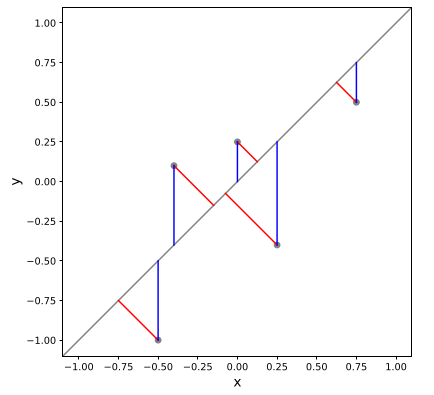
\includegraphics[width=0.3\textwidth]{unsupervisedLearning/PCA_linReg.png}
\caption{Zielfunktion von PCA minimiert die Summe der quadrierten Distanzen, orthogonal zur Geraden vs. Zielfunktion der linearen Regression, die Summe der vertikalen Abstände minimiert. PCA $\neq $ linReg!}
\end{figure}

Bei der \emph{linearen Regression} geht es um Funktionsapproximation, bei PCA um Dimensionsreduktion.\\

\underline{\textbf{Berechnung}}: Hauptkomponenten entsprechen den Eigenvektoren der Kovarianzmatrix der Datenpunkte. Die Eigenwerte geben die Varianz entlang der Hauptkomponenten an.
\begin{itemize}
    \item Kovarianzmatrix aufstellen: $Cov(E)=\frac{1}{m}\sum_{i=1}^{m} x^{(i)}(x^{(i)})^T$
    \item Kovarianzmatrix ist symmetrisch und positiv definit $\rightarrow$ Diagonalisierung möglich; es existieren genau \emph{n} reale Eigenwerte $\lambda_1\dots\lambda_n$ und Eigenvektoren $v_1\dots v_n$
    \item Eigenvektoren sind orthogonal zueinander und normiert $\rightarrow$ bilden die Hauptkomponenten
\end{itemize}

\underline{\textbf{Evaluation}}:
\begin{itemize}
    \item Verwendung der Evaluationsmaße der eigentlichen Lernaufgabe; z.B. F1-Maß für Klassifikation $\rightarrow$ aufwendig, da Datensätze verschiedener Dimensionalität gebildet und verglichen werden müssen
    \item besser: Messung des Verlustes an Varianz (wie verstreut sind die Datenpunkte \emph{E} im Raum?) durch Dimensionsreduktion $\rightarrow$ Wähle die Dimensionalität, bei der der Verlust an Varianz \emph{nicht zu hoch} ist $rightarrow$ hier muss Model nicht neu gelernt werden.
    \item Varianz der Datenpunkte: $var(E)=\frac{1}{m}\sum_{i=1}^{m}\|x^{(i)}\|^2$
    \item Retained Variance: $retVar(E^\text{compressed}, E)=\frac{var(E^\text{compressed})}{var(E)}$ $\rightarrow$ Anteil der Varianz von $E$, der in $E^\text{compressed}$ erhalten bleibt; es gilt stets $var(E^\text{compressed})\leq var(E)$.
    \item Wähle die Dimensionalität so klein wie möglich, so dass $retVar(E^\text{compressed}, E) \geq  \alpha$ für $\alpha\in [0,1]$. Typischerweise wird $\alpha\in[0.9,0.99]$ gewählt.
\end{itemize}
